\documentclass[11pt,a4paper]{article}

\usepackage[utf8]{inputenc}
\usepackage[T1]{fontenc}
\usepackage{lmodern}
\usepackage[margin=2.4cm]{geometry}
\usepackage{microtype}
\usepackage{parskip}
\usepackage{graphicx}
\graphicspath{{../../figures/cautionary/}}
\usepackage{amsmath,amssymb}
\usepackage{booktabs}
\usepackage{caption}
\usepackage{xcolor}
\usepackage{enumitem}
\usepackage[colorlinks=true,linkcolor=blue,citecolor=blue,urlcolor=blue]{hyperref}
\usepackage{authblk}

\title{\bfseries A control framework for topological data analysis of perturbation
single-cell RNA-seq: dispersion-matched nulls, traversal tests, and a drug-tolerance
case study}
\author[1]{H.-T.\ Lin}
\author[1]{Y.-H.\ Tu}
\affil[1]{\small Preprint --- methods / cautionary report. Code: \url{https://github.com/htlin222/sctda-cancer-plasticity}}
\date{\today}

\newcommand{\maxh}{\ensuremath{\max\text{-}H_1}}

\begin{document}
\maketitle

\begin{abstract}
\noindent Persistent homology is increasingly applied to single-cell RNA-seq (scRNA-seq)
to detect ``cyclic'' or non-tree-like cell-state structure, with the maximum degree-1
persistence (\maxh) used as a scalar readout of cell-state plasticity. We show that this
statistic, computed without structure-aware controls, conflates genuine topology with two
mundane confounds---transcriptional dispersion and the cell cycle---and we provide a reusable
four-part control framework that separates them: (i)~a \textbf{covariance-matched Gaussian
null} that distinguishes real structure from dispersion; (ii)~a \textbf{circular-coordinate
traversal test} that asks whether a detected ``loop'' is actually occupied before any cyclic
interpretation; (iii)~\textbf{cell-cycle regression evaluated within the dispersion-controlled
frame}, which we show is necessary because the common control (raw \maxh{} preserved after
regression) is inadequate; and (iv)~\textbf{bootstrap directional testing}, because \maxh{}
point estimates are subsample-unstable. On synthetic data with known ground truth the framework
is sensitive (it passes a genuine traversed loop) and specific (it rejects benign dispersion and
non-Gaussian non-cyclic structure). Applied as a worked case study to five longitudinal
EGFR-mutant lung-cancer systems, the framework decomposes an apparently compelling, cross-system,
drug-associated \maxh{} signal: cells never traverse the loop (Rayleigh $R \ge 0.965$ vs $0.881$
for a 12\%-occupied control), baseline \maxh{} equals a dispersion-matched null in every system,
the in-vitro drug excess is contributed by proliferating cells and vanishes after cell-cycle
regression, and the in-vivo (PDX) excess is genuine non-cell-cycle structure that nonetheless
still fails the traversal test. In no system does \maxh{} evidence a cell-traversed cycle.
\end{abstract}

\paragraph{Contributions.}
\begin{enumerate}[leftmargin=1.4em,itemsep=1pt]
\item A \textbf{covariance-matched Gaussian null} for \maxh{} separating genuine structure from
transcriptional dispersion, superseding the field-standard within-cell gene-shuffle null.
\item A \textbf{circular-coordinate traversal test} establishing occupancy of a persistent loop
as a precondition for any ``cyclic'' claim.
\item The observation and correction that the \textbf{common cell-cycle control (raw \maxh{}
preserved after S/G2M regression) is inadequate}, because raw \maxh{} is dispersion-dominated.
\item A \textbf{synthetic benchmark} characterising sensitivity and specificity, and a
five-system cancer \textbf{case study} of a confounded signal that is reproducible, cross-scale,
and wrong.
\end{enumerate}

\section{Introduction}
Topological data analysis (TDA), and persistent homology in particular, is an increasingly
popular lens on scRNA-seq. Its appeal is the ability to detect closed, non-tree-like structure
(loops; degree-1 homology, $H_1$) that trajectory-inference tools, designed for one-directional
progressions, are not built to quantify. In cancer drug tolerance this is attractive:
lineage-tracing studies show drug-tolerant persister cells reversibly transition among
transcriptional states, a behaviour naturally described as ``cyclic.'' A common move is to
summarise the topology with a single scalar, \maxh, and to read its increase under drug as a
measure of cyclic plasticity.

This inherits a known hazard. Persistent homology on a noisy high-dimensional point cloud reports
$H_1$ features whether or not the population occupies or traverses a loop, and \maxh{} as a scalar
conflates genuine structure with two confounds: transcriptional dispersion (the variance/spread of
the embedding, which directly inflates Vietoris--Rips persistence) and the cell cycle, which is
itself intrinsically a loop (G1$\to$S$\to$G2M$\to$G1). Cautionary methods work has repeatedly
shown that single-cell analyses require structure-aware nulls---for doublets, ambient RNA, batch
effects, and over-interpreted pseudotime---and topological summaries are no exception. Yet the
nulls in common use for scTDA (within-cell gene shuffles) do not control for dispersion, and
cell-cycle controls are typically evaluated on raw persistence rather than relative to a
dispersion baseline. We provide a control framework that makes both confounds explicit, validate
it on synthetic ground truth, and apply it to five EGFR-mutant lung-cancer systems.

\section{Results}

\subsection*{The control framework}
The framework takes a cell-by-PC embedding for each condition and reports three quantities plus a
decision rule. (1)~\emph{Dispersion test:} the ratio of observed \maxh{} to that of a multivariate
Gaussian matched to the embedding's mean and covariance; a ratio near 1 means the statistic is
explained by dispersion, a ratio robustly $>1$ indicates structure beyond dispersion.
(2)~\emph{Traversal test:} the Rayleigh concentration $R$ of circular coordinates from the
most-persistent $H_1$ class; $R$ near 1 means the population sits at one angle (loop not occupied).
(3)~\emph{Cell-cycle test:} the dispersion ratio recomputed after S/G2M-score regression. All three
are wrapped in bootstrap subsampling. Decision rule: \emph{structure beyond dispersion} if the
Gaussian ratio is robustly $>1$; \emph{a traversed loop} only if additionally $R<0.6$;
\emph{cell-cycle driven} if the excess does not survive S/G2M regression.

\subsection*{The framework is sensitive and specific on synthetic ground truth}
We validated the framework on point clouds where the answer is known (Fig.~\ref{fig:bench}). A
pure Gaussian blob gives ratio 0.93, $R=0.99$ (correctly \emph{no structure}). A uniformly
traversed loop gives ratio 8.35, $R=0.42$ (correctly a \emph{traversed loop}; sensitivity). A
sparse non-closed arc gives ratio 1.54 but $R=0.96$ (correctly \emph{structure, not traversed}).
Two well-separated Gaussian clusters---non-Gaussian but non-cyclic---give ratio 0.93 (correctly
\emph{no structure}; specificity): the Gaussian null does \emph{not} false-positive on benign
non-Gaussianity, the key objection to a covariance-matched null. A second non-parametric
dispersion-preserving null (independent per-PC permutation) agrees and is more conservative.

\subsection*{Case study: an apparent topological signal of drug tolerance}
We computed \maxh{} (top-30 PCs, $\mathbb{F}_2$) on five EGFR-mutant systems. \maxh{} increased
with drug in the osimertinib cell line and PDX models (osimertinib D0$\to$D14: $1.41\to3.78$;
PDX YU-006 untreated$\to$residual: $2.79\to5.46$; Fig.~\ref{fig:disp}), the kind of trend that
motivates scTDA applications. The erlotinib series is a counter-example---weak and non-monotonic
(D9 1.77, D11 1.08, the lowest of the series)---which we keep in view as evidence of instability.

\subsection*{Control 1 --- cells do not traverse the loop}
Circular coordinates collapse to a single angle in every cohort: Rayleigh $R \ge 0.965$
(Fig.~\ref{fig:ctrl}a)---more concentrated than the $R=0.881$ of a 12\%-occupied positive control.
Using Watermelon lineage barcodes, clonal lineages are if anything \emph{more} concentrated than
random groups. The persistent loop is a sparse feature the population does not occupy or traverse.

\subsection*{Control 2 --- baseline \maxh{} is dispersion}
Against the covariance-matched Gaussian null, baseline \maxh{} does not exceed dispersion
(osimertinib D0/D3 ratio $\approx 0.9$; observed $>$ null in 18--31\% of subsamples;
Fig.~\ref{fig:disp}). An excess appears only under drug (osimertinib D7/D14 in 100\%/98\%; PDX
residual 99\%). The field-standard gene-shuffle null, by destroying all covariance, tests only
``is there any structure,'' not ``structure beyond dispersion.'' The Gaussian null's failure mode
is conservative for our negative conclusion.

\subsection*{Control 3 --- the in-vitro excess is the cell cycle; the in-vivo excess is not}
Localising the cells contributing the osimertinib D14 excess (leave-one-cluster-out), the
structure-driving population is proliferating cells (DE: PTTG1, UBE2S, CKS1B, MYBL2; proliferation
markers MKI67/PCNA/CCNB1/CDK1/BIRC5, 5/6; EMT 1/19). In the pooled embedding, the excess does not
survive S/G2M regression: the D14 ratio falls 1.18$\to$0.99 and D14$>$D0 holds in only 31\% of
bootstraps (Fig.~\ref{fig:ctrl}b). This exposes a methodological error: the usual control reports
\emph{raw} \maxh{} preserved after regression, but raw \maxh{} is dispersion-dominated; the
cell-cycle contribution is visible only as a ratio to the dispersion null. The framework
decomposes rather than uniformly debunks: in the in-vivo PDX the residual-disease excess (the
strongest in the study) is \emph{not} cell cycle---excluding cycling cells leaves it intact
(G1-only ratio 2.07, 90\% CI $[1.37,2.61]$, $>1$ in 100\% of bootstraps). Yet this structure still
fails the traversal test ($R=0.965$): even where structure is real, the population does not
traverse it, so the ``cyclic plasticity'' reading remains unsupported. Across all five systems:
dispersion accounts for the baseline; the cell cycle for the in-vitro excess; the in-vivo residual
is genuine but non-traversed---and in no system does \maxh{} evidence a cell-traversed cycle.

\subsection*{A confound-resistant clonal statistic is under-powered}
We defined clonal state-memory $M(t)=1-H_{\mathrm{obs}}/H_{\mathrm{null}}$ against a lineage-shuffle
null. A baseline reduction is \emph{suggested} but not robust (M(D0) point estimate 0.48, 90\% CI
$[-0.05,0.29]$), and its decay under drug is not robust: the sign flips across clustering settings
(positive in 3/9), the trajectory is non-monotonic, and a depth-stratified null halves it
(Fig.~\ref{fig:mem}). The cause is power: only 12--33 clones with $\ge 3$ cells per timepoint.
Clonal-memory statistics require clone-rich designs current drug-timecourse datasets rarely provide.

\subsection*{Beyond rejection: the framework isolates a genuine, interpretable program}
A control framework earns trust only if it passes real structure as well as rejecting confounded
structure (cf.\ the synthetic true positive). The PDX residual is the worked example: its excess
is the one signal surviving every control, and the structure-driving cells (leave-one-cluster-out)
are a coherent multiciliated airway-epithelial program (PIFO, RSPH1, CFAP45/126/157, CAPS/CAPSL,
CETN2, TPPP3; secretory AGR2/AGR3). It is drug-emergent in YU-006---0.1\% of untreated cells but
9.6\% under residual disease ($\approx$6 $\to$ $\approx$187 cells in absolute terms while the
tumour contracts threefold)---consistent with the differentiated lineage states EGFR-TKI
persisters are known to adopt. The framework thus isolates genuine structure and localises it to
an interpretable state, not merely subtracts artefacts. Two bounds: the program is model-specific
(absent in YU-003), and copy-number inference could not resolve tumour-derived
(transdifferentiation) vs an expanded non-malignant population without a matched-normal reference.
And this real structure still fails the traversal test ($R=0.965$): even genuine structure is not
a traversed cycle.

\section{Methods}
\textbf{Datasets:} GSE134839, GSE150949 (Watermelon), GSE243562 (PDX), GSE131907, and the
EGFR-mutant subset of Maynard et al.\ 2020; standard scanpy QC/normalisation/HVG/PCA (seed 42),
subsampled to 1{,}000--1{,}500 cells. \textbf{Persistent homology:} \texttt{ripser} 0.6,
Vietoris--Rips to $H_1$ on top-30 PCs, $\mathbb{F}_2$. \textbf{Dispersion null:} draws from
$\mathcal{N}(\hat\mu,\hat\Sigma)$ of the PCA cloud; ratio $=$ observed/median(null); 30 bootstrap
subsamples with 90\% CIs; second null by per-PC permutation. \textbf{Traversal test:}
\texttt{dreimac} \texttt{CircularCoords} (DSPVJ), Rayleigh $R$; validated on a noisy circle
($R=0.12$) and a 12\%-occupied loop ($R=0.88$). \textbf{Cell-cycle test:} leave-one-cluster-out,
Wilcoxon DE with recovered gene symbols, S/G2M regression with the dispersion ratio bootstrapped.
\textbf{Synthetic benchmark:} four 1{,}200-cell scenarios, structure in 2-D embedded in 30-D with
isotropic noise. \textbf{Code:} \texttt{scripts/16\_*.py}--\texttt{scripts/25\_*.py} (MIT).

\section{Discussion}
A cross-system topological signal of drug tolerance---rising \maxh---is largely explained by
transcriptional dispersion and, in vitro, by the cell cycle; where genuine non-confound structure
remains (in-vivo PDX), it still does not evidence cyclic plasticity, because the population does
not traverse it. This is a cautionary, methodological contribution in the established lineage of
structure-aware single-cell controls. The biology of persister-state plasticity, established by
lineage tracing, is not in question; we show that static persistent-homology summaries do not
capture it and instead track nuisance variation. We recommend that topological claims on
perturbation scRNA-seq be accompanied, at minimum, by a dispersion-matched null, a traversal test,
cell-cycle regression in the dispersion-controlled frame, and bootstrap directional testing.

\paragraph{Outlook.} The framework's ability to isolate (not just reject) structure points to a
constructive use: the drug-emergent multiciliated program it surfaced in PDX residual disease is a
candidate tolerant-cell state. Establishing it as a discovery would require resolving cell-of-origin
(matched-normal CNV or EGFR-driver genotyping), reproduction in further models or patient
residual-disease specimens, and functional testing of whether the differentiated state confers
tolerance---a prospective, experiment-bearing programme rather than a reanalysis.

\paragraph{Limitations.} The cell-cycle attribution is demonstrated on the osimertinib cell line;
the PDX residual excess is shown to be non-cell-cycle but its positive identity is not established
here. We address \maxh; the dispersion null derives from the same filtration and is expected to
apply to other persistence summaries (persistence images, Adams et al.\ 2017; landscapes, Bubenik
2015) and higher-degree homology, though we do not test this. Traversal is inferred from snapshot
circular-coordinate concentration plus the clonal-spread proxy, not direct temporal observation.

\begin{figure}[t]\centering
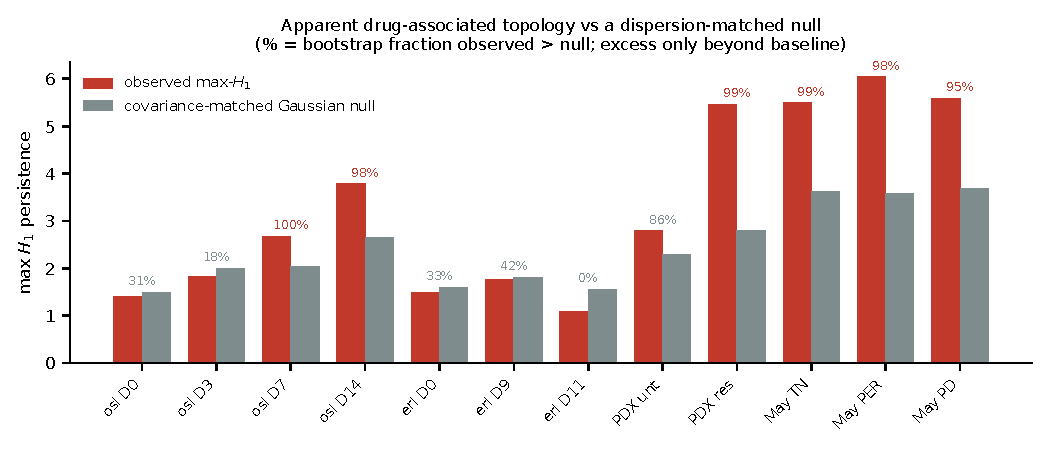
\includegraphics[width=\linewidth]{fig1_dispersion_null.pdf}
\caption{Observed \maxh{} vs a covariance-matched Gaussian (dispersion) null across five systems.
Percentages: bootstrap fraction observed $>$ null. Excess appears only under drug.}
\label{fig:disp}\end{figure}

\begin{figure}[t]\centering
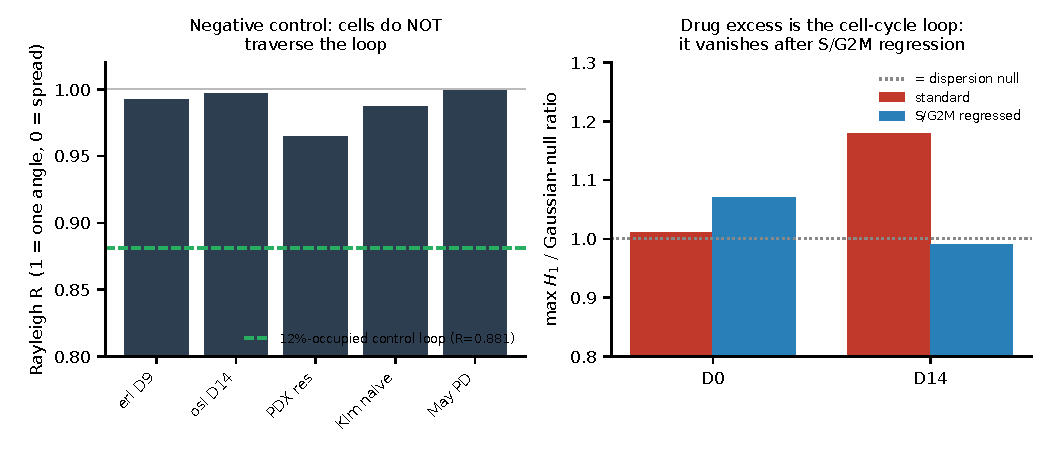
\includegraphics[width=\linewidth]{fig2_controls.pdf}
\caption{(a)~Traversal test: Rayleigh $R\ge0.965$ in all cohorts vs $0.881$ for a 12\%-occupied
control---cells do not traverse the loop. (b)~The in-vitro drug excess vanishes after S/G2M
regression.}
\label{fig:ctrl}\end{figure}

\begin{figure}[t]\centering
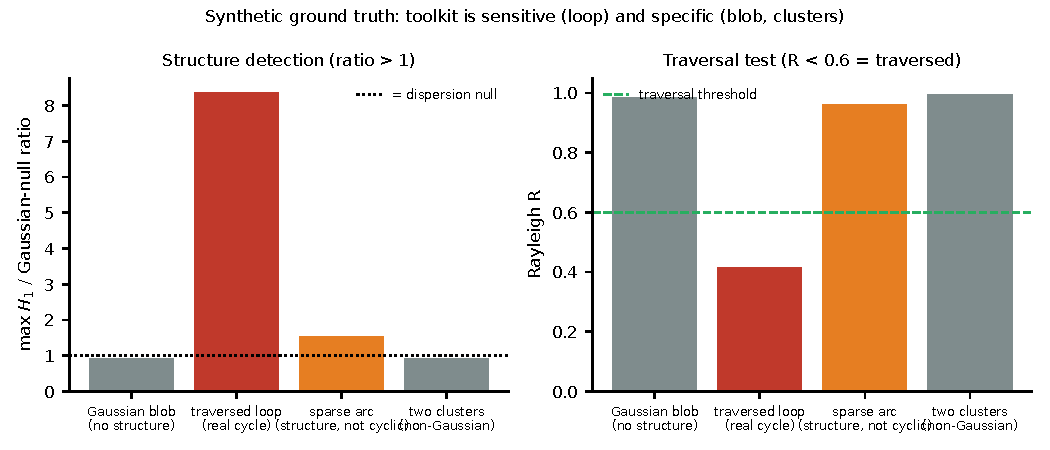
\includegraphics[width=\linewidth]{fig4_synthetic_benchmark.pdf}
\caption{Synthetic ground truth: the framework is sensitive (passes the traversed loop) and
specific (rejects the Gaussian blob and the two-cluster non-Gaussian case).}
\label{fig:bench}\end{figure}

\begin{figure}[t]\centering
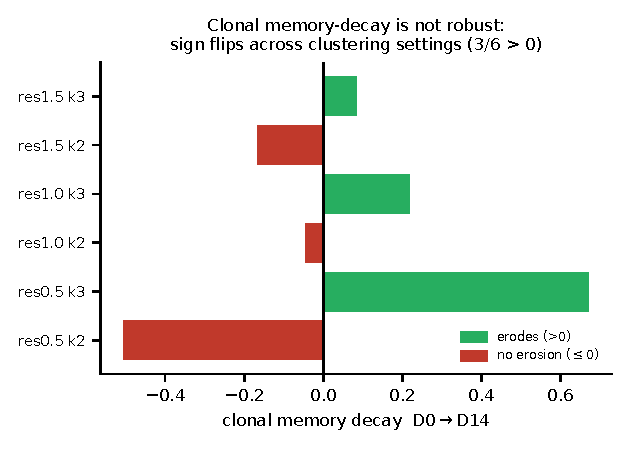
\includegraphics[width=0.62\linewidth]{fig3_memory_nonrobust.pdf}
\caption{Clonal memory-decay is not robust: the sign of the D0$\to$D14 change flips across
clustering settings.}
\label{fig:mem}\end{figure}

\end{document}
